\documentclass[11pt]{article}

\usepackage{amsmath}
\usepackage{amssymb}

\usepackage{graphicx}
\usepackage{tikz}

\usepackage{ytableau}

\title{Trees, \\ Math 4707, Spring 2021}
\date{}

\begin{document}


\maketitle

\vspace{-1cm}

\thispagestyle{empty}

An \emph{isomorphism} between graphs $G$ and $H$ is a one-to-one correspondence between the vertices of $G$ and of $H$ such that two vertices in $G$ are joined by an edge if and only if their corresponding vertices in $H$ are. If there is an isomorphism between $G$ and $H$ then we say that they are \emph{isomorphic}.

\begin{enumerate}

\item If $T$ is a tree and $G$ is isomorphic to $T$, must $G$ also be a tree?

\item What's the biggest collection of pairwise non-isomorphic trees on $4$ vertices you can find? On $5$ vertices? If you're feeling bored: on $6$?

\end{enumerate}

The \emph{degree sequence} $(d_1, d_2, \ldots, d_n)$ of a graph $G$ on $n$ vertices is the sequence of degrees $\mathrm{deg}_G(v)$ for all vertices $v$ of $G$, written in non-increasing order: $d_1\geq d_2 \geq \cdots \geq d_n$.

\begin{enumerate}

\setcounter{enumi}{2}

\item Explain why isomorphic trees have the same degree sequences.

\item Find two non-isomorphic trees with the same degree sequences.

\item Explain why the degree sequence $(d_1, d_2, \ldots, d_n)$ of a tree $T$ on $n$ vertices is a non-increasing sequence of integers between $1$ and $n-1$ such that $\sum_{i=1}^{n} d_i = 2(n-1)$.

\item {\bf Challenge}: show that any non-increasing sequence $(d_1, d_2, \ldots, d_n)$ of integers between $1$ and $n-1$ with $\sum_{i=1}^{n} d_i = 2(n-1)$ is the degree sequence of a tree on $n$ vertices.

\end{enumerate}

Recall that a \emph{spanning tree} of a connected graph $G$ is a subgraph that's a tree which contains all the vertices of $G$.

\begin{enumerate}
\setcounter{enumi}{6}
\item Find all the spanning trees of:
\[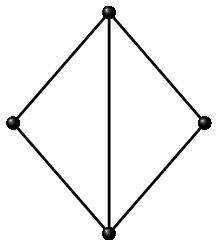
\includegraphics[width=1in]{kite.png}\]
\end{enumerate}

\end{document}
